% vim: set ts=2 sw=2 noet spell:

\chapter{Implementation} \label{chp:implementation}

\section{Overview}

First the tools used in this project are introduced. Then implementations of the transmitter and receiver chains is explained. Subsequently simulations and measurements of fading channels with an empirically computed bit error rate (BER) are presented. Finally, the issues and the state of our current implementation is discussed.

\section{Software Stack}

\subsection{GNU Radio}

For both the signal processing and the simulations the GNU Radio (GR) toolkit was chosen, as it already had drivers for the USRP hardware. GR is an open-source free software framework that can be used to build signal processing chains and software defined radios (SDR). GR is composed of two parts: a C\texttt{++} library with Python bindings to write signal processing code, and GNU Radio Companion (GRC), a graphical user interface to more easily construct signal processing chains by representing signal processing algorithms as ``blocks'' that are chained together with arrows, essentially drawing a diagram called ``flow graph''. An example of a flow graph is shown in \figref{fig:flowgraph}.

Internally GR works by keeping multiple memory buffers of samples, that are passed as pointers to the signal processing algorithms' ``work functions''. When the signal processing is complete, the output buffer of one block is given to the next block as input according to how they were connected in the flow graph. The structure of a block is shown in the Python listing \ref{lst:gr-block-py}. To improve performance GR creates a thread for each work function to parallelize the workload of the concurrently running signal processing blocks. For more details see the GNU Radio Wiki and User Manual in \cite{GRWiki}.

\begin{figure}
	\caption{
		A GNU Radio flow graph.
		\label{fig:flowgraph}
	}
\end{figure}

{\newcommand{\placeholder}[1]{\textit{\(\langle\)\,\textrm{#1}\,\(\rangle\)}}
\begin{lstlisting}[
	language = python, escapechar = {`}, float,
	caption = {A minimal GNU Radio block in Python.},
	captionpos = b, label = {lst:gr-block-py}
]
class myblock(gr.sync_block):
	# there are also other types of blocks such as interpolators 
	# (more outputs that inputs), decimators (more inputs than 
	# outputs) sync blocks have a 1-to-1 input to output ratio
	def __init__(self, `\placeholder{parameters}`):
		gr.sync_block.__init__(self, name="My Block",
			# this block as one input port and one output port
			# with samples that are 64 bit complex numbers
			in_sig=[np.complex64], out_sig=[np.complex64]
		)

	def work(self, inputs, outputs):
		# signal processing goes here
		# inputs and outputs are k x n arrays, where each
		# of the k rows is a port that contains n samples
		return `\placeholder{N of inputs that were processed}`
\end{lstlisting}}

\subsection{Dear PyGUI}\label{sec:GUI}

\begin{figure}
	\centering
	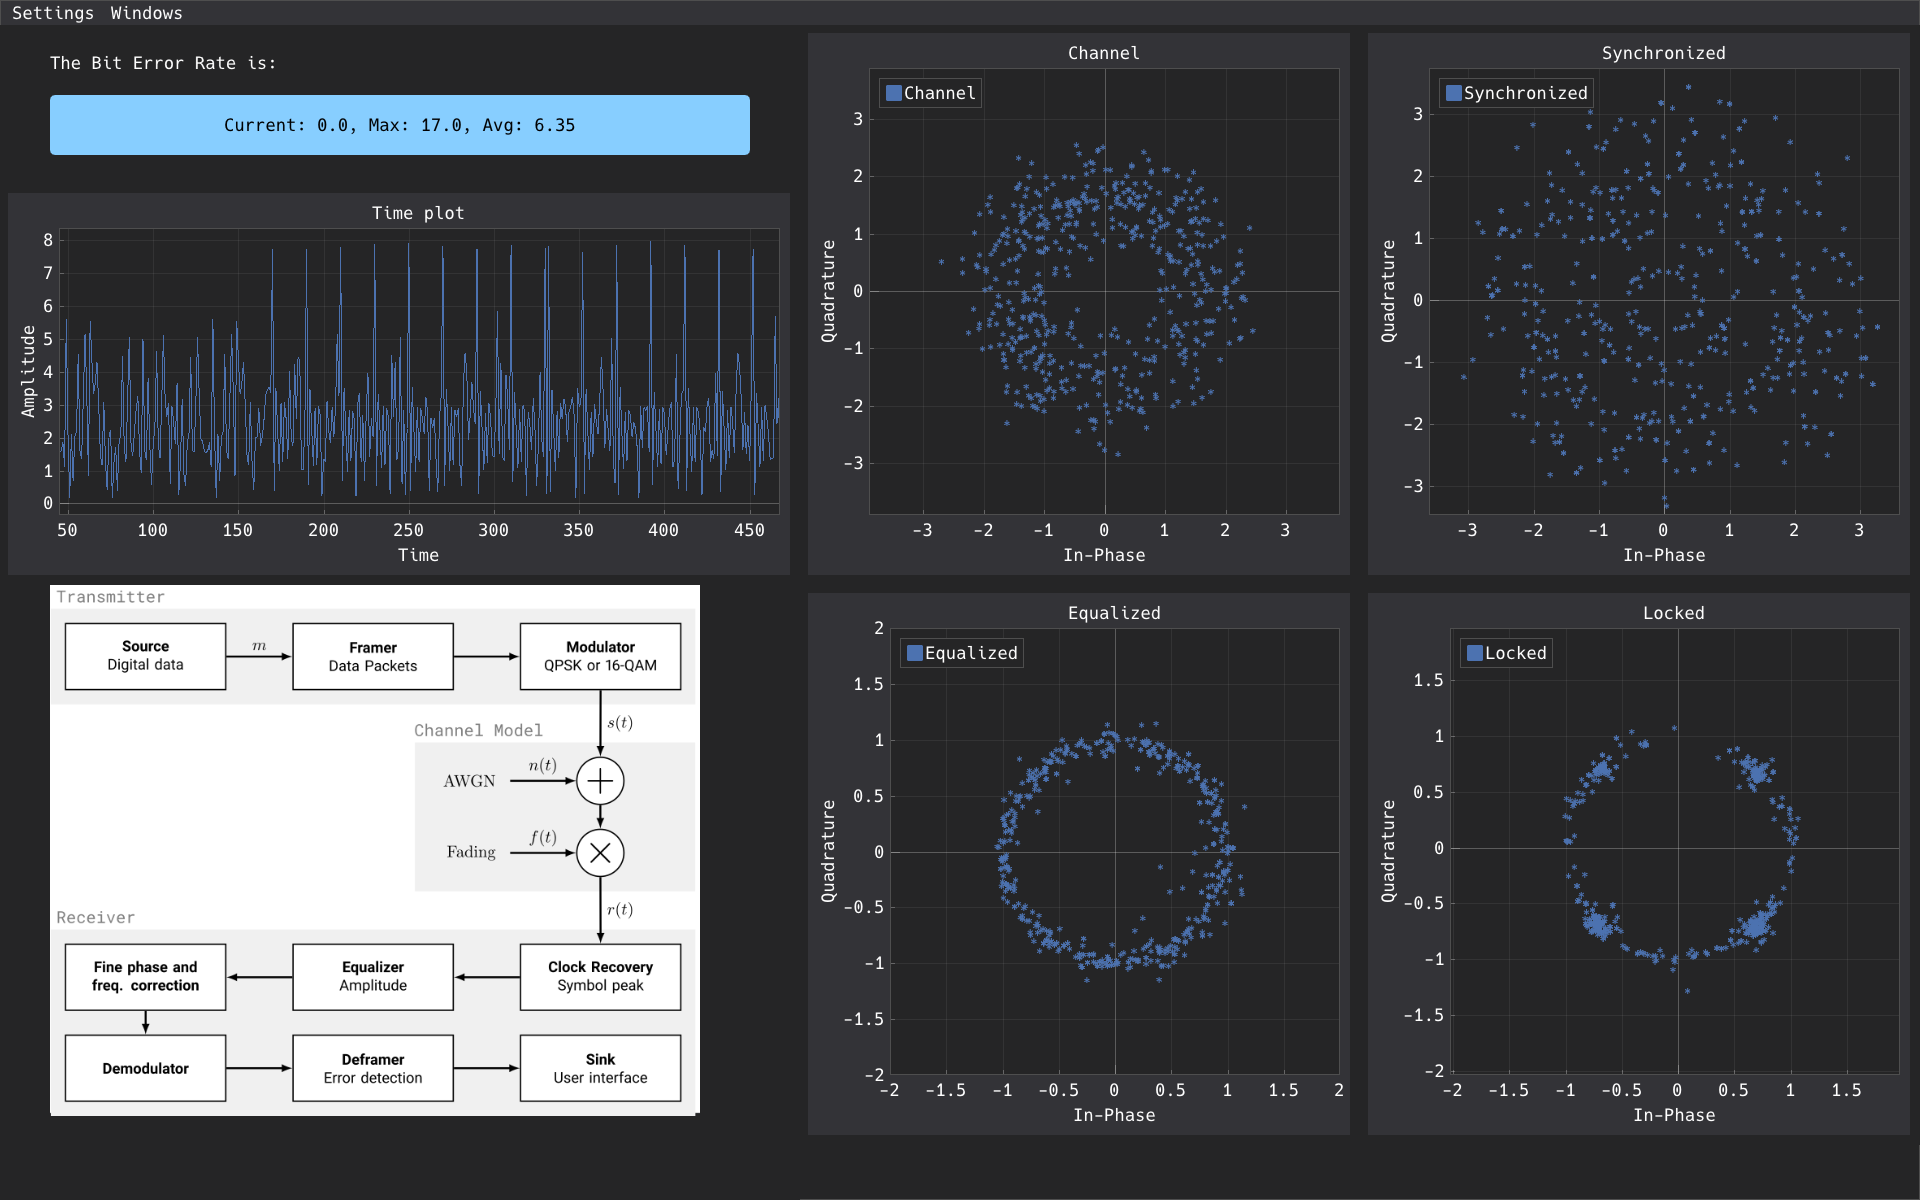
\includegraphics[frame, width = \linewidth]{figures/screenshots/gui_screenshot}
	\caption{Screenshot of the graphical interface of receiver built using the DearPyGUI library.}
\end{figure}

To construct a graphical interface for a demonstration platform the Dear IMGUI (immediate mode graphical user interface) library was chosen, mainly for its ease of use, wide range of techincal capabilites and high refresh rate. Dear PyGUI (DPG) are the Python bindings for the Dear IMGUI library.

The DPG GUI communicates with the GR flow graphs using the IP/UDP protocol. This decision to separate the project into two parts that communicate over the IP network was made because it is not very easy to extend the graphical interface of GRC without interfering with the sophisticated multi-threaded architecture of GR. Furthermore, this allows to have multiple correctly configure flow graph on disk and to choose which one to run and display on the graphical interface, instead of having a single flow graph whose parameters need to be changed each time. As a side effect, in theory this setup allows to have one computer running the graphical interface, and another remote machine running just the flow graph.

\section{Hardware}

As receivers and transmitter devices for the SDR setup two USRP B210 devices from Ettus Research were used. Some technical specifications are shown in \tabref{tab:usrp-specs}. GR provides off the shelf blocks that interface with the official API provided from Ettus Research.

\begin{table}[h]
	%TODO sepzifikationen ampssen / genauer? https://www.ettus.com/wp-content/uploads/2019/01/b200-b210_spec_sheet.pdf
	% https://kb.ettus.com/B200/B210/B200mini/B205mini#FAQ
	\centering
	\begin{tabular}{ll}
		\toprule
		Dimensions               & \(9.7 \times 15.5 \times 1.5\) cm \\
		Ports                    & 2 TX, 2 RX, Half or Full Duplex   \\
		RF frequencies           & 70MHz to 6GHz                     \\
		Bandwidth                & 200kHz -- 56MHz                   \\
		External reference input & 10 MHz                            \\
		\bottomrule
	\end{tabular}
	\caption{USRP B210 specifications \cite{EttusUSRPB210}. \label{tab:usrp-specs}}
\end{table}

\section{Transmitter chain}

\subsection{Data frame} \label{sec:data-frame}

\begin{figure}
\centering
% vim:ts=2 sw=2:
\begin{tikzpicture}[
		brace/.style = {
			decorate,
			decoration = {
				calligraphic brace,
				amplitude = 3mm,
				raise = 1mm,
				mirror,
			},
			very thick,
			pen colour = {black} 
		},
	]
	\matrix[
		column sep = -1pt,
		nodes = {
			draw, rectangle, very thick,
			minimum height = 12mm,
			text width = 20mm,
			align = center,
		},
	]{
		\node[] {Preamble \\ \(k\) Bytes}; &
		\node[fill=lightgray!20] (pad) {Padding \\ 1 Bit}; &
		\node[fill=red!10] (id) {ID \\ 5 Bits}; &
		\node[fill=red!10] {Length \\ 21 Bits}; &
		\node[fill=red!10] (par) {Parity \\ 5 Bits}; &
		\node[] {Payload \\ \(\ell\) Bytes}; \\
		% \node{Padding }; \\
	};

	\draw[brace] (id.south west) --
		node[midway, below = 5mm] {(31, 26) Hamming ECC}
		(par.south east);

	% \draw[brace] (par.north east) --
	% 	node[midway, above = 5mm] {4 Bytes}
	% 	(pad.north west);

\end{tikzpicture}

	\caption{
		Structure of framed data packets used in the implementation.
		\label{fig:dataframe}
	}
\end{figure}

To compute the empirical bit error rate (BER) of the setup, the data has to be framed by the transmitter and the bitstream needs to be synchronized on the receiver side. The structure of a data packet used in the implementation is shown in \figref{fig:dataframe}. A frame begins with an user specified \(k\)-byte preamble, that in the current implementation serves as synchronization pattern. Another use case for the preamble sequence could be to introduce channel estimation pilot symbols. Following the preamble are 4 bytes encoded using a (31, 26) Hamming code (plus 1 padding bit), that contain metadata about the packet, namely payload ID and payload length. Because the payload length in bytes is encoded in 21 bits, the theoretical maximum payload size is 2 MiB, which together with 32 possible unique IDs gives a maximum data transfer with unique frame headers of 64 MiB. These constraints are a result of decisions made to keep the implementation simple. % TODO: explain why its simpler this way


\subsection{Modulation}

GR provides a constellation modulator block, that already implements several standard constellations (QPSK and 16ary-QAM being of interest for us). The block also already integrates a root raised cosine filter, whose phase bandwidth (roll-off factor) can be given as parameter; in all flow graphs the roll off factor is \(\alpha = 0.35\).

\section{Receiver chain}

\subsection{Envelope detector}

What is here referred to as envelope detector has the purpose of synchronizing the symbols and equalizing the input signal amplitude. This is accomplished in GRC using two blocks: a polyphase clock sync and a constant modulus adaptive (CMA) filter equalizer. The input signal for the envelope detector has 4 samples per symbol, while the output has only one sample per symbol. The choice of the CMA equalizer later turned out to be a mistake in the QAM flow graphs, as it only works for envelope with a constant amplitude. In the latest version least mean square decision-directed (LMS-DD) equalizers have been used.

% \paragraph{Polyphase Clock Sync}
% %TODO : nochmals anschauen ob dieese erklärung verständlich ist und richtig interpretiert wurde.
% With the the polyphase clock sync the symbols can be synchronized by preforming a time synchronization with the help of multiple filterbanks. For that the derivative of the filtered signal should be minimized which turns to a better SNR. 
% This works with the help of two filterbanks, one of them contains the filters of the signal adapted to the pulse shaping with several phases. The other contains its derivative. So in the time domain it has a sinc shape, for the output Signal the sinc peak should be on a sample, with the fact that sinc(0) = 1 and sinc(0)' = 0 an error signal can be generated which tells how far away from the peak it is. This error Signal should be zero this is possible with the help of a loop second order whish constants the number of the filterbank and the rate. This rate is generated because of the clock difference between the transmitter and receiver to synchronized the receiver the filter goes through the phases. For the output one sample per symbol is enough.

% \paragraph{Equalizer}
% \skelpar[2]{CMA equalizer.}

\subsection{Frame synchronization and phase correction} \label{sec:phasecorr}

Once the envelope's clock is synchronized in the processing chain the data stream has one sample per symbol. At this point it is necessary to find where each data frame starts or end in order to correctly decode their payloads. For such purpose a special sequence called \emph{access code} is put in front of each frame. Access codes are sequences of samples that are carefully constructed to have an autocorrelation with a high peak at zero, and that rapidly decreases for increasing shifts. In other words, the autocorrelation of an access code high only when the sequence is perfectly aligned. Thus, by cross correlating an envelope signal \(r(t)\), that periodically contains an access code \(a(t)\) with the access code itself, and looking for peaks in the result, it is possible to determine where each frame begin. Furthermore, by analyzing the values of the peaks it is possible to extract information about the phase and frequency offsets.

To understand how correlation peaks allow for fine phase correction, recall that the cross correlation (denoted here by \(\star\)) of two complex valued signals is
\begin{equation}
	R_{ra}
	= (r \star a)(t)
	= \int_\mathbb{R} r(\tau) a^*(\tau - t) \,d\tau
	= r(t) * a^*(-t),
\end{equation}
which is equivalent to a convolution, with the left term being time-reversed complex conjugated \cite{Gallager}. This last property is especially useful because it makes possible to implement cross correlation using FIR filters. Some interesting properties of the cross correlation are that correlation with itself (autocorrelation) at \(t = 0\) is
\begin{equation}
	R_{aa} = (a \star a)(0)
	= \int_\mathbb{R} a(\tau) a^*(\tau - 0) \,d\tau
	= \int_\mathbb{R} |a(\tau)|^2 \,d\tau \in \mathbb{R},
\end{equation}
which is a real number. And more importantly the correlation with an out of phase copy \(a'(t) = a(t) e^{j\varphi}\) at 0 is
\begin{equation} \label{eqn:xc-oop-copy}
	% R_{a'a} =
	(a' \star a)(0) 
	= \int_\mathbb{R} a(\tau)e^{j\varphi}  a^*(\tau) \,d\tau
	= R_{aa} e^{j\varphi}.
\end{equation}
The relevant observation to make in \eqref{eqn:xc-oop-copy} that since \(R_{aa}\) is a real number, the phase of the cross correlation at \(t = 0\) is the phase of \(a'(t)\). This fact can be exploited to implement fine phase correction for the received envelope in relatively few steps as follows:
\begin{enumerate}
	\item Compute the cross correlation \(R_{ra}\) of the envelope \(r(t)\) with the access code \(a(t)\),
	\item Find the maximum value of \(\hat{R}_{ra} = \max R_{ra}(t)\) (correlation peak),
	\item Extract the phase offset \(\varphi = \arg \hat{R}_{ra}\),
	\item Remove the phase offset in the envelope by multiplying it with the complex conjugate of the offset, that is \(\hat{r}(t) = r(t) e^{-j\varphi}\).
\end{enumerate}

\subsubsection{Implementing fine phase and frequency correction} \label{sec:implement-phasecorr}

To implement in GR what was discussed in section \ref{sec:phasecorr} two blocks shown in \figref{fig:phasecorr-blocks} were used: a correlator estimator block, and a custom block. The former essentially implements the first 3 of the steps discussed at the end of section \ref{sec:phasecorr}. The correlator estimator block is given a sequence of samples, and when the cross correlation between them and the input stream is higher than a certain threshold (90\% of the amplitude of a perfect autocorrelation), it produces a ``tag'' in the output stream, that contains the phase estimate.

Tags are GR's way of working with metadata that is attached to a sample. Internally tags are just polymorphic data structures containing a number indicating the absolute offset (in samples), and a pair of arbitrary values called ``key'' and ``value''. Tags are passed on from one block to the next like sample streams (unless the block specifies to do otherwise).

Thus, the tagged stream is processed with a custom block, of which a simplified version of its work function shown in listing \ref{lst:phasecorr-work}. The custom block also implements fine frequency correction (shown in listing \ref{lst:phasecorr-blockphase}) by linearly interpolating the phase estimates between each pair of tags (called chunk). This can be rather trivially be formulated for a chunk of \(N\) samples with the
\begin{subequations}
	\begin{align}
		k\text{-th chunk digital frequency} \quad  & \Omega_k = (\varphi_{k+1} - \varphi_k) / N, \text{ and the }\\
		k\text{-th chunk phase estimate} \quad & \Phi(n) = \varphi_k - \omega_k n/N.
	\end{align}
\end{subequations}

\subsubsection{Performance of the implementation}\label{sec:preforming-implementation}

The phase and frequency correction block was implemented with the design goal of being able to correct under ideal conditions a maximal frequency offsets of \(\hat{\epsilon} = 0.1\%\), which is sufficient to take into account small Doppler shifts at walking speed (\(v = \SI{2}{\meter\per\second}\)) with carrier at \(f_c = 2.4\) GHz. The USRP B210 devices have an internal clock frequency accuracy of \(\epsilon = 1\text{ ppm} = 10^{-6}\), which results in a total frequency offset of
\begin{equation}\label{eq:doppler}
	\Delta f = f_c \left( \frac{v}{c_0} + \epsilon \right)
	= \SI{2.4}{\giga\hertz} \left(
		\frac{\SI{2}{\meter\per\second}}{\SI{3e8}{\meter\per\second}} + 10^{-6} 
	\right) = \SI{2416}{\hertz}.
\end{equation}
Because the frequency estimate is linearly interpolated, the phase error may not exceed \(\pi\) (half rotation) during one data frame (chunk). These constraints imply that for frames of \(N'\) symbols of duration \(T\) each, using \(\kappa\) samples per symbol the relation
\begin{equation}\label{Doppler-shift}
	2\pi\Delta f N' T \kappa \leq \pi
	\implies T = 1/f_s \leq \frac{1}{2\Delta f N' \kappa},
	\iff N' \leq \frac{1}{2\Delta f T \kappa},
\end{equation}
must hold. By further setting \(\kappa = 4\) and \(N' = 32\) we obtain a minimum sampling frequency of approximately \(\SI{618.5}{\kilo\hertz}\), or conversely by letting \(f_s = \SI{1}{\mega\hertz}\) we have a maximum frame length of \(N' = 51\) symbols. In other words, roughly every 50 symbols the system must send an access code sequence. This result is rather unfortunate as it requires a lot more processing power than expected.

\begin{figure}
	\centering
	% TODO: move code into separate file
	% vim: set ts=2 sw=2 noet:
\begin{tikzpicture}[
		blk/.style = {
			draw, rectangle, thick, black,
			minimum width = 15mm,
			minimum height = 3mm,
			outer sep = 1mm,
			pattern = vertical lines,
			pattern color = lightgray,
		},
	]

	\foreach \i in {0,1,...,4}{
		\coordinate (blkC\i) at (15mm*\i,0);
		\node[blk] (blk\i) at (blkC\i) {};
		\node[below] (phi\i) at (blk\i.south west) {\(\varphi_{\i}\)};
	}
	% last phase 
	\node[below] (phi5) at (blk4.south east) {\(\varphi_{5}\)};

	% first block
	\node[blk, minimum width = 10mm, xshift = 2.5mm, fill = red!30] (S) at (-15mm,0) {};
	\node[anchor = east] at (S.west) {Input};

	% last block
	\node[blk, minimum width = 9mm, xshift = -3mm, fill = blue!30] (E) at ($(blk4)+(15mm,0)$) {};

	% labels
	\draw[thick, latex-] (blk3.north) to[out = 90, in = 180] ++(5mm,6mm)
		node[right] {Chunk of \(N\) samples};

	\draw[thick, latex-] (blk0.north east) ++(-1mm,0) to[out = 90, in = 0] ++(-5mm,6mm)
		node[left] (tags) {Phase tags};
\end{tikzpicture}

	\caption{
		Graphical representation of the input samples for the work function of the fine phase and frequency correction block (shown in listing \ref{lst:phasecorr-work}). Roughly every \(N\) samples there is a tag containing the information of the phase error (computed using the cross correlation peak). The white `chunks' of samples can be corrected using their respective left and right tag values. The samples in the red chunk need phase information from the previous block processing. The samples in the blue chunk need a phase information from the future, which is not attainable. Thus for the blue chunk the frequency estimate of the previous chunk is used.
		\label{fig:phasecorr-chunks}
	}
\end{figure}


\begin{lstlisting}[
	texcl = true, language = python, escapechar = {`},
	float, captionpos = b, label = {lst:phasecorr-work},
	caption = {
		Simplified work function of fine phase correction block that corrects only samples `in the middle'. The version that is actually used does handle edge cases that have been removed here for readability. See also \figref{fig:phasecorr-chunks} for a graphical representation of the inputs and listing \ref{lst:phasecorr-blockphase} for the definition of the \texttt{block\_phase} function.
	},
]
def work(self, inputs, outputs):
	# alias for inputs of the first port
	inp = inputs[0]
	# read phase tags from stream
	is_phase = lambda tag: pmt.to_python(tag.key) == "phase_est"
	tags = filter(is_phase, self.get_tags_in_window(0, 0, len(inp)))
	# create a list of pairs \(((\varphi_0,\varphi_1), (\varphi_1, \varphi_2), \ldots, (\varphi_{k-1}, \varphi_k)))\)
	pairs = zip(tags, tags[1:])
	# compute phase correction between each pair of tags
	chunks = [self.block_phase(start, end) for (start, end) in pairs]
	# flatten array to get \(\Phi(n)\) and compute the correction
	phases = np.concatenate(chunks)
	correction = np.exp(-1j * phases) 
	# write to the first output port
	left = tags[0].offset - self.nitems_written(0)
	right = tags[-1].offset - self.nitems_written(0)
	outputs[0][left:right] = inp * correction
	# return how many samples were processed
	return len(outputs[0])
\end{lstlisting}

\begin{lstlisting}[
	texcl = true, language = python, escapechar = {`},
	float, captionpos = b, label = {lst:phasecorr-blockphase},
	caption = {
		Block phase function referenced in listing \ref{lst:phasecorr-work}.
	},
]
def block_phase(self, start, end):
	# compute number of samples between tags
	nsamples = end.offset - start.offset
	# unpack pmt values into start and end phase
	sphase = pmt.to_python(start.value)
	ephase = pmt.to_python(end.value)
	# compute frequency offset between start and end
	phasediff = (ephase - sphase)
	freq = phasediff / nsamples
	if phsediff > np.pi:
		phasediff -= np.pi
	elif phasediff < -np.pi:
		phasediff += np.pi
	# compute chunk values
	return sphase * np.ones(nsamples) + freq * np.arange(0, nsamples)
\end{lstlisting}

\section{Channel simulations}

In order to study the effects of multipath fading, a series of simulations have been made under different conditions. To simulate a channel affected by multipath fading two blocks from the GR library, and a third custom block were used. The channel model can simulate AWGN, a frequency offset and either a Rayleigh (NLOS) oder Rice (LOS) fading.

\subsection{Fading with discrete time model} \label{sec:discrete-time-model-fir}

For the statical version according to \ref{sec:discrete-time-model} for implement and illustrate the fading effect, a separate block was created and implemented in the channel. Nearer shown in \ref{lst:fractional-delay-fir}. This block is based on a FIR filter. It can be displayed with a direct path (LOS) or without one (NLOS).
With the help of this filter, the delay of the line of side paths are illustrated. In this block it is possible to simulate any number of these paths with different strengths, as long as there is an associated amplitude specified for each delayed ray. 

A special case is show in \figref{fig:qpsk-simulations-static}, where the delay in sample is the same as the sample per symbol value or a multiple of it. An other example is shown in the same figure,with more diffident delayed paths, with the delay values of \texttt{[0.25,4,6.3,3.25]} and the amplitude values of \texttt{[0.2,0.5,0.4,0.08]}.
Unfortunately, these simulation values do not correspond to the reality, because too many incalculable side effects occur, which aren't possible to illustrate in this simulation.

This block was additionally implemented with the method described in \ref{sec:fractional-delay} to allow non-integer delay values compared to the samples shown in \figref{fig:fractional-delay-sinc-plot}. Where the sinc function does not select an integer sample. Which in turn means that the other sampled values do not add up to zero.
Thus, they will be distributed among the other whole numbers. A window function could also be implemented to limit these values. Here none was implemented because the sinc function is restricted.

\begin{lstlisting}[
	texcl = true, language = python, escapechar = {`},
	float, captionpos = b, label = {lst:fractional-delay-fir},
	caption = {
		Implementation of a static fractional delay FIR filter.
	},
	]
	def work(self, input_items, output_items):
		inp = input_items[0]
		oup = output_items[0]
		# find the length of the highest order filter
		max_order = 2 * np.floor(np.max(self.delays)) + 1
		max_samples = np.arange(0, max_order +1)
		max_len = len(max_samples)
		# total impulse response (of all taps)
		tot_h = np.zeros(int(max_len))
		# compute for each tap
		for (a, d) in zip(self.amplitudes, self.delays):
			# compute fir coefficients
			order = 2 * np.floor(d) + 1
			samples = np.arange(0, order + 1)
			# compute impulse response
			h = a * np.sinc(samples - d)
			# correct length
			h = np.concatenate([h, np.zeros(max_len - len(h))])
			# add to other filters
			tot_h += h
		# add a LOS path if necessary
		tot_h[0] = self.los
		# compute output
		y = np.convolve(inp, tot_h)
		# add values from previous block processing
		y += np.concatenate([self.temp, np.zeros(len(y) - len(self.temp))])
		# write to output
		oup[:] = y[:len(inp)]
		# save rest for next block processing
		self.temp = y[len(inp):]
		return len(oup)
	
\end{lstlisting}

\subsection{Fading with statistical model}

In order to represent the effect of the multipaht fading not only statically, a second model was created using the Frequency Selective Fading Model from Gnu Radio, according to \ref{sec:statistical-model},which was implemented after the algorithm from the paper \cite{Alimohammad2009}, with the help of the sum-of sinusoid principal (SOS). The algorithm in this block is implemented with the aim that only a small number of sinusoids are needed. 
This number represent the sinusoids which are simulated for each ray, for the foaling simulations shown the value 8 has been chosen.

It can also be chosen whish statical model should be taken for the simulation Rayleigh or Rician. When the Rician model is taken also a realistic value for the factor \(K\) need to be given. Whish is something between zero and ten. As mentioned earlier, when  \(K=0\) the distribution is the same as with the Rayleight model. For a faktor \(K = 5.1\) the probability function is gaussien distributed.

The power delay profile which specify the delay in time for each impulse need to be in sample. For this delayed vector some realistic values are for the first delay \cite{Mathworks}, when theirs non line of side zero. The second delayed path depend on the environment of measurement. In an indoor environment it is usually between \(1\cdot10^{-9}\) to \(1\cdot10^{-7}\) and in an outdoor environment between \(1\cdot10^{-7}\) to \(1\cdot10^{-5}\). The rest depends on  the bandwidth. 

The magnitudes of the pulses are given with the linear value. In practices the avarage path gain of a fading path is in the range of \([ -20 \text{dB} , 0\text{dB}]\).

To add some movement, like a movable transmitter some Doppler shift can be initialized after the formula \eqref{Doppler-shift}. But it need to be normalized with the sampling rate. 
An example of such a simulation plot is shown in \figref{fig:qpsk-simulations-dynamic}.

When nothing mentioned the number of how many FIR- filter taps are used is eight.
%TODO: Should this be mentoned

\subsubsection{Issues}

Some difficulty was how to check the correction of the statistical models, if there is noise in the channel, from the fading effect, especially when the doppler frequency is included. This was difficult to recreate, when the parameter haven't the special case in which the the amplitude and the phase shift can be seen exactly. 
To have some indication to verified the plot, mainly whether the movement could be correct a little Matlab model was used with the same values for the different distributions.

%TODO: Other Plots?
\subsubsection{Real value example}

In order to obtain a realistic simulation the values for multipath fading propagation condition for a Extended Typical Urban (ETU) model, from the ETSI (European Telecommunication Standards Institute), where used\cite{ETSI}, with the values shown in \tabref{tab:etsi-tap-values}. For those the maximum Doppler frequency possibilities are predefined. In the following examples \figref{fig:dynamic-exp-real} either \(\SI{5}{\hertz}\) or \(\SI{70}{\hertz}\) were used, as in \eqref{eq:doppler} \(\SI{16}{\hertz}\) calculated for a walking speed of \(\SI{2}{\meter\per\second}\). Those predefined values had a speed of
\begin{equation}
	v = \frac{\Delta f}{f_c}\cdot c_0 = \frac{\SI{5}{\hertz}}{\SI{2.4}{\giga\hertz}}\cdot \SI{3e8}{\meter\per\second}= \SI{0.625}{\meter\per\second}
\end{equation}
and
\begin{equation}
	v = \frac{\Delta f}{f_c}\cdot c_0 = \frac{\SI{70}{\hertz}}{\SI{2.4}{\giga\hertz}}\cdot \SI{3e8}{\meter\per\second}= \SI{8.75}{\meter\per\second}
\end{equation}.

The numbers of tags used in this case are similar to the number of given values.
\skelpar[5]{
	More simulation plots. Beschreiben.
}

\begin{table}[b]
	\centering
	\begin{tabular}{rr}
		\toprule
		\bfseries Excess tap delay & \bfseries Relative power \\
		\midrule
		\SI{   0}{\nano\second} & \(\SI{-1.0}{\decibel} \approx 0.7943\) \\
		\SI{  50}{\nano\second} & \(\SI{-1.0}{\decibel} \approx 0.7943\) \\
		\SI{ 120}{\nano\second} & \(\SI{-1.0}{\decibel} \approx 0.7943\) \\
		\SI{ 200}{\nano\second} & \(\SI{ 0.0}{\decibel} = 1.0000\) \\
		\SI{ 230}{\nano\second} & \(\SI{ 0.0}{\decibel} = 1.0000\) \\
		\SI{ 500}{\nano\second} & \(\SI{ 0.0}{\decibel} = 1.0000\) \\
		\SI{1.6}{\micro\second} & \(\SI{-3.0}{\decibel} \approx 0.5011\) \\
		\SI{2.3}{\micro\second} & \(\SI{-5.0}{\decibel} \approx 0.3162\) \\
		\SI{5.0}{\micro\second} & \(\SI{-7.0}{\decibel} \approx 0.1995\) \\
		\bottomrule
	\end{tabular}
	\caption{Extended Typical Urban model (ETU) ETSI Standard PDP values for multipath fading propagation conditions \cite{ETSI}. \label{tab:etsi-tap-values}}
\end{table}

\subsection{Measurements/Demonstration}

\skelpar[5]{
	Do some masurements
}

\subsection{Empirical BER} \label{sec:ber}
To find out how accurate the simulations are comparer with a simulation of the fadinng effect and tested measurements, the byte error rate of the system is calculated. This is done with the help of a user specified \(k\)-byte test frame in the beginning of each vector. Implemented according to the code in \ref{lst:ber-work}. Every bit is compared with the test vector at the beginning before the modulation and demodulation part. 
Because of the fact that the test vector has some random bit at the end the bit error rate has always a value on average 32, even when its perfect match.  So to avoid high numbers this value is subtracted and only on focused on the positive values. 

The vector which is used as test vector is: \texttt{[0x1f, 0x35, 0x12, 0x48]}, because this numbers are well suited to compare.
For generating the byte error rate it is focus on byte-blocks of a specific length. So for each of this blocks compared with test vector there is a BER. To make it simpler or better said to avoid mistakes, the last 200 of this individual BER are taken to find an average and the highest value. 

\skelpar[5]{
	Maybe more 
}


\begin{lstlisting}[
	texcl = true, language = python, escapechar = {`},
	float, captionpos = b, label = {lst:ber-work},
	caption = {
		Custom block to compute the empirical BER.
	},
	]
	def work(self, input_items, output_items):
		# input is a list of blocks of k-bytes
		inp = input_items[0]
		# for each block
		for i in inp:
			i = np.array(i, dtype=np.uint8)
			# XOR to compute the difference
			v = np.array(self.vgl, dtype=np.uint8) ^ i
			# compute how many bits differ
			ber = sum(np.unpackbits(v))
			# save BER value
			self.ber_samples.appendleft(ber)
		# compute statistics and send to GUI
		ber_max, ber_min, ber_avg = self.ber_stats()
		self.send(self.encode([ber_max, ber_min, ber_avg]))
		return len(inp)
\end{lstlisting}

\section{Issues in the current implementation}

\subsection{Non modulated access codes}

Currently as described in section \ref{sec:data-frame}, the access codes are put as bytes in front of the frame in the \(k\)-byte preamble. For this to work, the access code bytes must still have a good autocorrelation function after being modulated into symbols using the chosen modulation scheme. This works well with QPSK, because the constellation is quite simple and the length of the sequence is only halved after the modulation (since QPKS has 2 bits per symbol). Thus, in the QPSK flow graph the longest known Barker sequence  \texttt{0x1f35} (13 bits, left padded with zeros) is sufficient (\(\approx 7\) symbols).

With QAM however, the complexity of the constellation and the higher number of bits per symbol makes it increasingly difficult to find binary sequences retain a good autocorrelation function after being modulated. A better solution would be to use for example a \emph{constant amplitude zero autocorrelation waveform} (CAZAC) of length \(N\), which is computed with
\begin{equation}
	u_k = \exp\left(j\frac{M\pi K}{N}\right) \text{ where }
	K = \begin{cases}
		k^2 & \text{when } N \text{ is even} \\
		k(k+1) & \text{when } N \text{ is odd}
	\end{cases},
\end{equation}
and \(M\) is relatively prime to \(N\) \cite{Chu1972}. CAZAC waveforms are ideal because they have a Dirac delta as autocorrelation \cite{Chu1972}, i.e. \(R_{uu}(\tau) = \delta(\tau)\). Though unfortunately, since these complex values are not on any constellation point they break some assumptions of the polyphase clock sync and the LMD DD equalizer (but not CMA). Thus to use CAZAC waveforms the transmitter needs to put them in front of the modulated symbols (for example using a correctly parametrized stream mux block in GR), and the receiver would need to synchronize with the sequence before the clock recovery or equalization. The latter is especially problematic because then it is no longer possible to identify the peak by comparing the autocorrelation value to a fixed threshold as done in section \ref{sec:implement-phasecorr}.

\subsection{Single threaded GUI application}

\subsection{Incomplete parts}

\subsection{Clock synchronization issues}

Unfortunately the SDR needs an external clock generator. For that a Rubidium Frequency STd. Model FS725 is used. Better said two of them, to make them more movable and independent, with the clock frequency \SI{10}{\mega\hertz}. Those Rubidiums where used, because the synchronization, dosn`t work as planed in \ref{sec:preforming-implementation}. 
%TODO: Right squenz?
Without those only the amplitudes could be seen in the Plots, with all the noise from the inter-symbol differences. 

\subsection{GUI Parameter change}

As in \ref{sec:GUI} described the GUI was implemented, but unfortunately the parts where the parameter could be changed, will showing the current simulation isn't possibl like the noise voltage of the channel or the bandwidth from the Polyphase Clock , the Gain of the Equalizer aren't implemented yet. Actually everything which needs a responds from the interfaces to the GR. 

The second part which is missing is to be able to change the timing plot for the different scattering plots.

% TODO : Picture of the setup
% TODO: Plots from the Hardware


\newgeometry{
	top = 25mm, bottom = 25mm,
	inner = 15mm, outer = 15mm,
}
% \section{Constellation plots}
\begin{figure}
	\centering
	\label{fig:qpsk-simulations-static}
	% vim: set ts=2 sw=2 noet:

\newcommand{\makeplot}[6]{%
	\hfill
	\begin{tikzpicture}
		\begin{axis}[
				width  = {\linewidth / 3.5},
				height = {\linewidth / 3.5},
				grid = major,
				xmin = {-#4}, xmax = {#4},
				ymin = {-#4}, ymax = {#4},
				#5
			]

			\addplot[only marks, #6] table[x index = #2, y index = #3] {#1};
		\end{axis}
	\end{tikzpicture}
	\hfill
}

\noindent
% \makeplot{figures/data/qpsk_sim_constellations_without_effects.dat}{0}{1}{4}{}
% \makeplot{figures/data/qpsk_sim_constellations_static.dat}{0}{1}{4}{}
\makeplot{figures/data/qpsk_sim_constellations_static_symb.dat}{0}{1}{4}{
	ylabel = {Channel with ISI},
	yticklabel style = {
		text width = 2.25em,
		align = right,
	},
	title = {},
}{magenta}
\makeplot{figures/data/qpsk_sim_constellations_static_symb_vec.dat}{0}{1}{4}{title = {},}{magenta}
\makeplot{figures/data/qpsk_sim_constellations_static_symb_NLOS.dat}{0}{1}{4}{title = {},}{magenta}
\newline

\noindent
% \makeplot{figures/data/qpsk_sim_constellations_without_effects.dat}{2}{3}{4}{}
% \makeplot{figures/data/qpsk_sim_constellations_static.dat}{2}{3}{4}{}
\makeplot{figures/data/qpsk_sim_constellations_static_symb.dat}{2}{3}{4}{%
	ylabel = {Synchronized},
	yticklabel style = {
		text width = 2.25em,
		align = right,
	},
}{magenta!80!blue}
\makeplot{figures/data/qpsk_sim_constellations_static_symb_vec.dat}{2}{3}{4}{}{magenta!80!blue}
\makeplot{figures/data/qpsk_sim_constellations_static_symb_NLOS.dat}{2}{3}{4}{}{magenta!80!blue}
\newline

\noindent
% \makeplot{figures/data/qpsk_sim_constellations_without_effects.dat}{4}{5}{1}{}
% \makeplot{figures/data/qpsk_sim_constellations_static.dat}{4}{5}{1}{}
\makeplot{figures/data/qpsk_sim_constellations_static_symb.dat}{4}{5}{1}{%
	ylabel = {Equalized},
	yticklabel style = {
		text width = 2.25em,
		align = right,
	},
}{magenta!60!blue}
\makeplot{figures/data/qpsk_sim_constellations_static_symb_vec.dat}{4}{5}{1}{}{magenta!60!blue}
\makeplot{figures/data/qpsk_sim_constellations_static_symb_NLOS.dat}{4}{5}{1}{}{magenta!60!blue}
\newline

\noindent
% \makeplot{figures/data/qpsk_sim_constellations_without_effects.dat}{6}{7}{1}{}
% \makeplot{figures/data/qpsk_sim_constellations_static.dat}{6}{7}{1}{}
\makeplot{figures/data/qpsk_sim_constellations_static_symb.dat}{6}{7}{1}{%
	ylabel = {Locked},
	yticklabel style = {
		text width = 2.25em,
		align = right,
	},
}{magenta!40!blue}
\makeplot{figures/data/qpsk_sim_constellations_static_symb_vec.dat}{6}{7}{1}{}{magenta!40!blue}
\makeplot{figures/data/qpsk_sim_constellations_static_symb_NLOS.dat}{6}{7}{1}{}{magenta!40!blue}
\newline


	\caption{
		Simulations of a static fading channel models with different tap values. The samples were generated using the custom block discussed in section \ref{sec:discrete-time-model-fir}. For the 1 tap model the fading tap was \(0.2\delta(n - 0.25)\), and for the 4 tap model uses \(0.2 \delta(n - 0.25) + 0.08 \delta(n - 3.25) + 0.5 \delta(n - 4) + 0.4 \delta(n - 6.3)\). In both cases the delays are given in samples.
		% delay = [0.25, 3.25, 4, 6.3]
		% ampl =  [0.2, 0.08, 0.5, 0.4]
	}
\end{figure}
\newpage
\begin{figure}
	\centering
	% vim: set ts=2 sw=2 noet:

\newcommand{\makeplot}[5]{%
	\hfill
	\begin{tikzpicture}
		\begin{axis}[
				width  = {\linewidth / 3.3},
				height = {\linewidth / 3.3},
				grid = major,
				xmin = {-#4}, xmax = {#4},
				ymin = {-#4}, ymax = {#4},
				colormap name=viridis,
				#5
			]

			\addplot[only marks, scatter] table [x index = #2, y index = #3] {#1};
		\end{axis}
	\end{tikzpicture}
	\hfill
}

% -------------------------------------------------------------------

\noindent
\makeplot{figures/data/qpsk_sim_dynamic_grblock_nlos_etsi_doppler5.dat}{0}{1}{4}{
	ylabel = {Channel with ISI},
	yticklabel style = {
		text width = 3em,
		align = right,
	},
	title = {NLOS, \(\Delta f = \SI{5}{\hertz}\)},
}
%
\makeplot{figures/data/qpsk_sim_dynamic_grblock_los_etsi_doppler5_k5.dat}{0}{1}{4}{
	title = {LOS, \(\Delta f = \SI{5}{\hertz}, K = 5\)},
}
%
\makeplot{figures/data/qpsk_sim_dynamic_grblock_los_etsi_doppler70_k5.dat}{0}{1}{4}{
	title = {LOS, \(\Delta f = \SI{70}{\hertz}, K = 5\)},
}
\newline

% -------------------------------------------------------------------

\noindent
\makeplot{figures/data/qpsk_sim_dynamic_grblock_nlos_etsi_doppler5.dat}{2}{3}{4}{%
	ylabel = {Synchronized},
	yticklabel style = {
		text width = 3em,
		align = right,
	},
}
\makeplot{figures/data/qpsk_sim_dynamic_grblock_los_etsi_doppler5_k5.dat}{2}{3}{4}{}
\makeplot{figures/data/qpsk_sim_dynamic_grblock_los_etsi_doppler70_k5.dat}{2}{3}{4}{}
\newline

% -------------------------------------------------------------------

\noindent
\makeplot{figures/data/qpsk_sim_dynamic_grblock_nlos_etsi_doppler5.dat}{4}{5}{2}{%
	ylabel = {Equalized},
	yticklabel style = {
		text width = 3em,
		align = right,
	},
}
\makeplot{figures/data/qpsk_sim_dynamic_grblock_los_etsi_doppler5_k5.dat}{4}{5}{2}{}
\makeplot{figures/data/qpsk_sim_dynamic_grblock_los_etsi_doppler70_k5.dat}{4}{5}{2}{}
\newline

% -------------------------------------------------------------------

\noindent
\makeplot{figures/data/qpsk_sim_dynamic_grblock_nlos_etsi_doppler5.dat}{6}{7}{2}{%
	ylabel = {Locked},
	yticklabel style = {
		text width = 3em,
		align = right,
	},
}
\makeplot{figures/data/qpsk_sim_dynamic_grblock_los_etsi_doppler5_k5.dat}{6}{7}{2}{}
\makeplot{figures/data/qpsk_sim_dynamic_grblock_los_etsi_doppler70_k5.dat}{6}{7}{2}{}
\newline

	\caption{
		Simulations with a dynamic fading channel model using PDP values of the Extended Typical Urban model (ETU) of the ETSI standard normative Annex B.2 in \cite{ETSI}. The color gradient represents progression in time.
		\label{fig:qpsk-simulations-dynamic}
	}
\end{figure}
\newpage
\begin{figure}
	\centering
	% vim: set ts=2 sw=2 noet:

\newcommand{\makeplot}[5]{%
	\hfill
	% \tikzset{external/force remake}
	\begin{tikzpicture}
		\begin{axis}[
				width  = {\linewidth / 3.3},
				height = {\linewidth / 3.3},
				grid = major,
				xmin = {-#4}, xmax = {#4},
				ymin = {-#4}, ymax = {#4},
				colormap name=viridis,
				#5
			]

			\addplot[only marks, scatter, point meta = \thisrow{samplenr}]
				table [x index = #2, y index = #3] {#1};
		\end{axis}
	\end{tikzpicture}
	\hfill
}

% -------------------------------------------------------------------

\noindent
\makeplot{figures/data/qam_sim_dynamic_grblock_nlos_etsi_doppler5.dat}{0}{1}{4}{
	ylabel = {Channel with ISI},
	yticklabel style = {
		text width = 3em,
		align = right,
	},
	title = {NLOS, \(\Delta f = \SI{5}{\hertz}\)},
}
%
\makeplot{figures/data/qam_sim_dynamic_grblock_los_etsi_doppler5_k5.dat}{0}{1}{4}{
	title = {LOS, \(\Delta f = \SI{5}{\hertz}, K = 5\)},
}
%
\makeplot{figures/data/qam_sim_dynamic_grblock_los_etsi_doppler70_k5.dat}{0}{1}{4}{
	title = {LOS, \(\Delta f = \SI{70}{\hertz}, K = 5\)},
}
\newline

% -------------------------------------------------------------------

\noindent
\makeplot{figures/data/qam_sim_dynamic_grblock_nlos_etsi_doppler5.dat}{2}{3}{4}{%
	ylabel = {Synchronized},
	yticklabel style = {
		text width = 3em,
		align = right,
	},
}
\makeplot{figures/data/qam_sim_dynamic_grblock_los_etsi_doppler5_k5.dat}{2}{3}{4}{}
\makeplot{figures/data/qam_sim_dynamic_grblock_los_etsi_doppler70_k5.dat}{2}{3}{4}{}
\newline

% -------------------------------------------------------------------

\noindent
\makeplot{figures/data/qam_sim_dynamic_grblock_nlos_etsi_doppler5.dat}{4}{5}{2}{%
	ylabel = {Equalized},
	yticklabel style = {
		text width = 3em,
		align = right,
	},
}
\makeplot{figures/data/qam_sim_dynamic_grblock_los_etsi_doppler5_k5.dat}{4}{5}{2}{}
\makeplot{figures/data/qam_sim_dynamic_grblock_los_etsi_doppler70_k5.dat}{4}{5}{2}{}
\newline

% -------------------------------------------------------------------

\noindent
\makeplot{figures/data/qam_sim_dynamic_grblock_nlos_etsi_doppler5.dat}{6}{7}{2}{%
	ylabel = {Locked},
	yticklabel style = {
		text width = 3em,
		align = right,
	},
}
\makeplot{figures/data/qam_sim_dynamic_grblock_los_etsi_doppler5_k5.dat}{6}{7}{2}{}
\makeplot{figures/data/qam_sim_dynamic_grblock_los_etsi_doppler70_k5.dat}{6}{7}{2}{}
\newline

	\caption{
		TODO QAM simulation
	}
\end{figure}
\begin{figure}
	\centering
	% vim: set ts=2 sw=2 noet:

\newcommand{\makeplot}[5]{%
	\hfill
	% \tikzset{external/force remake}
	\begin{tikzpicture}
		\begin{axis}[
				width  = {\linewidth / 3.3},
				height = {\linewidth / 3.3},
				grid = major,
				xmin = {-#4}, xmax = {#4},
				ymin = {-#4}, ymax = {#4},
				colormap name=viridis,
				#5
			]

			\addplot[only marks, scatter, point meta = \thisrow{samplenr}]
				table [x index = #2, y index = #3] {#1};
		\end{axis}
	\end{tikzpicture}
	\hfill
}

% -------------------------------------------------------------------

\noindent
\makeplot{figures/data/qpsk_hw_lab.dat}{0}{1}{.25}{
	ylabel = {Channel with ISI},
	yticklabel style = {
		text width = 3em,
		align = right,
	},
	title = {QPSK LOS, Indoors (Lab)},
}
%
\makeplot{figures/data/qpsk_hw_outdoors_1.dat}{0}{1}{.25}{
	title = {QPSK LOS, Outdoors},
}
%
\makeplot{figures/data/qam_hw_lab.dat}{0}{1}{2}{
	title = {QAM LOS, Indoors (Lab)},
}
\newline

% -------------------------------------------------------------------

\noindent
\makeplot{figures/data/qpsk_hw_lab.dat}{2}{3}{.25}{%
	ylabel = {Synchronized},
	yticklabel style = {
		text width = 3em,
		align = right,
	},
}
\makeplot{figures/data/qpsk_hw_outdoors_1.dat}{2}{3}{.25}{}
\makeplot{figures/data/qam_hw_lab.dat}{2}{3}{2}{}
\newline

% -------------------------------------------------------------------

\noindent
\makeplot{figures/data/qpsk_hw_lab.dat}{4}{5}{2}{%
	ylabel = {Equalized},
	yticklabel style = {
		text width = 3em,
		align = right,
	},
}
\makeplot{figures/data/qpsk_hw_outdoors_1.dat}{4}{5}{2}{}
\makeplot{figures/data/qam_hw_lab.dat}{4}{5}{2}{}
\newline

% -------------------------------------------------------------------

\noindent
\makeplot{figures/data/qpsk_hw_lab.dat}{6}{7}{2}{%
	ylabel = {Locked},
	yticklabel style = {
		text width = 3em,
		align = right,
	},
}
\makeplot{figures/data/qpsk_hw_outdoors_1.dat}{6}{7}{2}{}
\makeplot{figures/data/qam_hw_lab.dat}{6}{7}{2}{}
\newline

	\caption{
		TODO QPSK hardware
	}
\end{figure}
\newpage
\restoregeometry
